\documentclass[11pt,a4paper]{report}

\usepackage[margin=2.2cm]{geometry}
\usepackage{titlesec}
\usepackage{enumitem}
\usepackage{longtable}
\usepackage{array}
\usepackage{booktabs}
\usepackage{xcolor}
\usepackage{listings}
\usepackage{hyperref}
\usepackage{tikz}
\usepackage{tcolorbox}
\usepackage{fancyhdr}
\usepackage{parskip}
\usetikzlibrary{positioning,arrows.meta,shapes.geometric,fit,backgrounds}

\definecolor{codebg}{RGB}{245,245,245}
\definecolor{hpegreen}{RGB}{1,169,130}
\definecolor{darknavy}{RGB}{30,40,60}

\lstset{
  backgroundcolor=\color{codebg},
  basicstyle=\ttfamily\small,
  breaklines=true,
  frame=single,
  numbers=left,
  numberstyle=\tiny,
  columns=fullflexible,
  showstringspaces=false
}

\hypersetup{
  colorlinks=true,
  linkcolor=darknavy,
  urlcolor=hpegreen,
  citecolor=hpegreen
}

\pagestyle{fancy}
\fancyhf{}
\fancyhead[L]{ArchGuide Interview Preparation - Volume 2}
\fancyhead[R]{\thepage}
\renewcommand{\headrulewidth}{0.4pt}

\titleformat{\chapter}[display]
  {\normalfont\huge\bfseries\color{darknavy}}
  {\chaptertitlename\ \thechapter}{20pt}{\Huge}

\newtcolorbox{notebox}[1][]{colback=hpegreen!8,colframe=hpegreen!60!black,fonttitle=\bfseries,title={#1}}
\newtcolorbox{qabox}[1][]{colback=darknavy!5,colframe=darknavy!70,fonttitle=\bfseries,title={#1}}

\title{\Huge \textbf{ArchGuide Project} \\[0.4cm] \Large Complete Reverse-Engineering and Interview Preparation Guide \\[0.6cm] \large Volume 2 of 3: Security, Features, API Communication, State Management, Design Patterns, Algorithms, Performance, Scalability, Production Readiness and Engineering Tradeoffs}
\author{Prepared for Full-Time Offer Technical Interview Preparation \\ Hewlett Packard Enterprise (HPE)}
\date{\today}

\begin{document}

\maketitle
\tableofcontents

\chapter{Authentication and Security}

\section{Login and Signup Flow}

ArchGuide does not implement its own signup or login forms, password storage, or session database. Instead it delegates identity entirely to Firebase Authentication using the Google OAuth provider. The end to end flow is as follows:

\begin{enumerate}[leftmargin=*]
  \item The user clicks "Sign in with Google" inside the `AuthModal` component. The frontend lazily loads the Firebase client SDK (deferred so it never blocks the initial page render or the Largest Contentful Paint metric) and calls `signInWithGoogle()`, which opens Google's OAuth consent popup.
  \item Google authenticates the user and returns control to Firebase, which issues a signed ID token, a JSON Web Token (JWT) containing claims such as the user's UID, email, name, photo URL, and an expiry timestamp, all signed with Google's private key.
  \item The frontend's `auth-context.tsx` receives the authenticated user object through Firebase's `onAuthStateChanged` listener, updates global state, and immediately calls the backend's `/api/v1/users/sync` endpoint, sending the ID token as a Bearer token and the user's profile fields in the request body. This call is retried up to three times with exponential backoff (a fix tagged "FE-004") to tolerate transient network issues immediately after sign in.
  \item The backend's `users` router verifies the token using the Firebase Admin SDK, extracts the UID from the verified claims, checks that this UID matches the `uid` field in the request body (preventing one authenticated user from writing another user's profile, a fix tagged "SEC-001"), and performs an upsert into the `User` table, including an email based account linking path for the edge case where the same email address has previously been associated with a different UID (which can happen if a user signs in with different methods).
  \item From this point forward, every authenticated API request from the frontend includes the cached ID token as a Bearer token in the Authorization header. The backend's `verify_firebase_token` dependency verifies it on each request; there is no separate backend issued session token or cookie.
\end{enumerate}

\textbf{Guest mode:} a user may skip sign in entirely. In that case, the frontend generates a random UUID, prefixes it with "guest\_", and stores it in `localStorage`; this synthetic identifier is sent as the `user_id` for project creation, and the backend treats any `user_id` beginning with "guest\_" as an anonymous, unauthenticated identity that requires no token verification, but is also not linked to any real account and exists only in that browser's local storage (and, for sessions without a project, directly in the database without ownership restrictions).

\section{Session Management and Token Handling}

ArchGuide is a stateless backend with respect to authentication: it does not store server side sessions, does not issue its own tokens, and does not use cookies for authentication. Every request must carry a valid Firebase ID token, and the backend's only job is to verify that token's cryptographic signature, expiry, and claims on each request, an approach often called "stateless JWT authentication." The frontend's `auth-token.ts` module implements an in-memory cache for the current ID token with a four minute time to live (deliberately shorter than Firebase's roughly one hour token expiry, to ensure the cached token is always refreshed well before it could expire mid request) and deduplicates concurrent token requests through a shared, in-flight promise, so that if five components simultaneously need a token, only one actual call to Firebase is made and all five await the same result.

\begin{qabox}[Likely Interview Questions]
\textbf{Q: Why did you choose stateless JWT verification over server side sessions?} \\
A: It removes an entire category of infrastructure and operational concerns, no session store to provision, replicate, or evict from, and it scales horizontally without any need for sticky sessions or shared session state across backend instances, since any instance can independently verify any token using only Google's public keys. The tradeoff is that a JWT cannot be instantly revoked before its natural expiry (server side sessions can be deleted immediately); Firebase mitigates this with relatively short token lifetimes (about one hour) and the option to revoke refresh tokens, which the client SDK handles by silently obtaining a fresh ID token. \\[4pt]
\textbf{Q: Where is the password stored?} \\
A: Nowhere in this application. Google handles authentication entirely; ArchGuide never sees, transmits, receives, or stores a password. This eliminates the single largest class of authentication related data breach risk for the application's own infrastructure, though it does mean the application's security is now partially dependent on Google's, a tradeoff that is overwhelmingly favorable for a project at this scale.
\end{qabox}

\section{Authorization Model}

Authentication (proving who you are) and authorization (deciding what you are allowed to do) are distinct concerns, and ArchGuide implements its own authorization layer on top of Firebase's authentication. The rules, enforced primarily in the `analysis` and `projects` routers, are:

\begin{itemize}[leftmargin=*]
  \item A `Session` that has no associated `Project` (a guest questionnaire run, or a guest document upload with no project context) is viewable by anyone who knows its analysis id; this is an intentional design choice reflecting that such sessions carry no account linkage and the analysis id itself (a UUID) is effectively a capability token.
  \item A `Session` belonging to a project whose `user_id` begins with "guest\_" is similarly viewable by anyone with the analysis id, since "guest\_" projects are, by definition, not tied to any verified identity.
  \item A `Session` belonging to a project owned by an authenticated user requires the requester's verified Firebase UID to match the project's `user_id`; any mismatch results in an authorization error, regardless of whether the requester is authenticated as some other user or not authenticated at all.
\end{itemize}

This logic is centralized in a single helper function, `_check_session_ownership()`, rather than being duplicated (and potentially inconsistently re-implemented, with subtle bugs) across every endpoint that touches session data, an application of the Don't Repeat Yourself principle directly motivating better security posture.

\section{Encryption}

Transport level encryption (HTTPS/TLS) is provided by the hosting platforms (Vercel for the frontend, Railway for the backend, and the managed database, cache, and vector store providers), not implemented by the application itself, which is the correct and standard approach; implementing your own TLS termination would be both unnecessary and risky. At rest, the managed providers (Supabase, Upstash, Qdrant Cloud, Firebase) handle encryption of stored data as part of their service guarantees. The application does not store any data, such as passwords or payment details, that would require additional application level encryption beyond what these providers already supply.

\section{Common Web Vulnerabilities and How They Are Mitigated}

\begin{longtable}{p{3.0cm}p{9.4cm}}
\toprule
\textbf{Vulnerability} & \textbf{Mitigation present in this codebase} \\
\midrule
\endhead
Cross-Site Scripting (XSS) & React escapes all dynamically rendered text content by default, preventing injected HTML or script from executing; the application does not use `dangerouslySetInnerHTML` for user supplied content. The backend's `SecurityHeadersMiddleware` additionally sets a `Content-Security-Policy` header, which provides a second, defense in depth layer that would limit the damage of any XSS that somehow occurred (for example, by restricting which script sources the browser will execute). \\
Cross-Site Request Forgery (CSRF) & CSRF specifically targets cookie based authentication, where a browser automatically attaches credentials to cross site requests. Because ArchGuide uses Bearer tokens in an explicit Authorization header (which browsers do not attach automatically to cross origin requests the way they do cookies), the classic CSRF attack vector does not apply in the same way. CORS is also configured to accept requests only from known origins. \\
SQL Injection & All database access goes through SQLAlchemy's ORM and parameterized query construction; the codebase contains no raw, string-concatenated SQL built from user input anywhere in the routers or services, which is the standard and correct way to prevent this class of vulnerability entirely. \\
NoSQL Injection & Not directly applicable, since the relational data store is PostgreSQL, but the same discipline (no untrusted input used to construct queries dynamically) extends to the Redis cache key construction (keys are built from session ids and fixed prefixes, not raw user input) and Qdrant's payload filters (filtered strictly by session id, a server generated UUID). \\
Path Traversal & The upload router explicitly sanitizes uploaded filenames before using them in any filesystem path: it strips backslashes, rejects sequences containing "..", and removes null bytes (a fix tagged "SEC-3.1"), preventing an attacker from crafting a filename such as "../../etc/passwd" to write or read outside the intended upload directory. \\
Denial of Service via oversized payloads & The PDF export endpoints validate their request bodies against an `ExportRequest` Pydantic schema with explicit maximum lengths (for example, sixty four characters for an analysis id, twenty entries for a ranking list), tagged "SEC-007," preventing an attacker from submitting an enormous payload designed to exhaust memory or CPU during PDF generation. The upload endpoint similarly enforces a fifty megabyte file size ceiling. \\
Replay Attacks & Firebase ID tokens are time bounded (roughly one hour) and bound to specific audience and issuer claims that the Admin SDK verifies; an intercepted token cannot be replayed indefinitely, and the short client side cache (four minutes) further limits the window during which a captured token would remain useful from the application's perspective. The application does not implement a nonce based replay defense of its own, relying on Firebase's token model, an acceptable choice for its threat model but worth acknowledging as a boundary of the system's own security guarantees. \\
Token Theft / Impersonation & The `/users/sync` endpoint cross checks the JWT's verified UID against the UID claimed in the request body (fix "SEC-001"), preventing a scenario where a stolen or forged request body could impersonate a different user even with a validly signed token for someone else. Project update schemas exclude the `user_id` field entirely, making ownership immutable after creation (fix "SEC-002") and closing off a class of "reassign this resource to myself" attacks. \\
Information Disclosure via the AI assistant & The chat router applies a hardcoded, regular-expression based safety gate (`_is_unsafe()`) that intercepts and refuses, before any LLM call is made, requests that attempt to extract API keys, system prompts, or backend implementation details, providing a deterministic backstop independent of the underlying model's own alignment. \\
Cache Poisoning Across Users & The analysis endpoint performs the ownership check before consulting the Redis cache (fix "SEC-008"), specifically to prevent a scenario where one user's cached result could be served to a different, unauthorized user who happened to guess or otherwise obtain the session id. \\
Insecure Logging & The codebase replaced raw `print()` statements used for authentication initialization failures with proper structured logging (fix "SEC-004"), ensuring that failures are captured by production log aggregation systems (where they can be alerted on) rather than being silently lost in a container's standard output that nobody is watching. \\
Improper CORS Configuration & The CORS middleware is configured to never simultaneously set `allow_credentials=True` and `allow_origins=["*"]`, a combination that violates the CORS specification's intent and can expose authenticated endpoints to any origin (fix "SEC-3.5"). \\
\bottomrule
\end{longtable}

\begin{qabox}[Likely Interview Questions]
\textbf{Q: If an attacker obtained a valid analysis id for someone else's guest session, what could they see?} \\
A: They would be able to view that analysis's results, because guest sessions are intentionally not access controlled beyond possession of their UUID, which functions as a capability token. This is a deliberate tradeoff: requiring an account for every analysis would add friction that conflicts with the product's "try it instantly, no signup required" value proposition, and the UUID's effectively unguessable 128 bit space makes brute forcing infeasible. The boundary of this design is that it depends on the analysis id never being inadvertently exposed (for example, in a referrer header to a third party site, or in a publicly indexed location); a more conservative design might add a short lived, signed access token to guest analysis URLs, which would be a reasonable hardening step to propose if asked how to improve this. \\[4pt]
\textbf{Q: What is the single most important security decision in this codebase, and why?} \\
A: Centralizing the session ownership check in `_check_session_ownership()` and ensuring it always runs before any cache lookup. Authorization bugs are uniquely dangerous because they fail silently from the attacker's perspective, the system appears to work normally, just for the wrong person, and they are uniquely easy to introduce inconsistently when the same logic is copy-pasted across multiple endpoints. Centralizing it in one place, and ordering it correctly relative to the cache (cache-then-check would have leaked data; check-then-cache does not), closes off an entire category of "I checked ownership in endpoint A but forgot in endpoint B" bugs at the source.
\end{qabox}

\chapter{Feature by Feature Breakdown}

For each major feature this section gives functional and non-functional requirements, implementation notes, the data flow, edge cases, failure scenarios, and interview style questions with strong answers.

\section{Feature: Document Upload Analysis}

\textbf{Functional requirements:} accept PDF, DOCX, and TXT files up to fifty megabytes; extract text with page level granularity where possible; reject documents that are not architecture related; extract ten signals with confidence and source attribution; produce a ranked recommendation.

\textbf{Non-functional requirements:} the end to end pipeline should complete within roughly one to three minutes for typical documents (the frontend's polling cap reflects this expectation); the system should degrade gracefully rather than fail outright if any single stage (vector indexing, a specific LLM provider) is unavailable; no user's document content or extracted signals should ever be visible to another user.

\textbf{Data flow:} browser to `/api/v1/upload` (multipart, with optional Bearer token) to filename sanitization and ownership check to `Session` row creation (status "processing") to `DocumentParser.parse()` to `validate_document_relevance()` to (in parallel or in sequence depending on configuration) vector indexing into Qdrant and `SignalExtractor` based extraction to confidence gating to `ScoringEngine.score()` and `sensitivity_analysis()` to `cost_analysis` computation to `followup_generator` question generation to persistence of `Signal` and `Result` rows to Redis caching to `AnalysisResponse` returned to the browser, and finally synchronous cleanup of the temporary uploaded file.

\textbf{Edge cases handled:}
\begin{itemize}[leftmargin=*]
  \item A scanned, image only PDF with no extractable text, the relevance gate's minimum word count check rejects it with a clear, actionable message.
  \item A document that is itself a previously generated ArchGuide report, the circular upload detector recognizes characteristic phrases and structure and rejects it, preventing a confusing "analysis of an analysis" loop.
  \item Fewer than three signals extracted with confidence above 0.35, the "confidence gate" flags the result as having insufficient data, and the response includes a `data_sufficient: false` indicator so the frontend can display an appropriate warning rather than presenting a low confidence recommendation as if it were authoritative (fix tagged "AI-5.2").
  \item All extracted signals' source quotes concentrated on a single page of a multi-page document, a "signal concentration warning" is raised, since this pattern often indicates the LLM anchored on one easily parsed section and may have missed information elsewhere in the document.
\end{itemize}

\textbf{Failure scenarios and recovery:} if parsing fails entirely (a corrupted file), the session is marked "error" with a user facing explanation. If vector indexing fails, the pipeline continues without it (a "non-fatal" design choice, since signal extraction can still proceed using the raw filtered text, just without retrieval augmentation). If the server crashes mid-pipeline, the startup recovery logic finds the orphaned "processing" session on the next boot and marks it "error," so the user is not left waiting forever.

\section{Feature: Guided Questionnaire Analysis}

\textbf{Functional requirements:} present up to ten multiple choice questions; convert answers directly into signals; produce the same caliber of recommendation as the document path, without requiring a document.

\textbf{Why it exists alongside document upload:} not every user has a ready made requirements document, and even those who do may want a faster, more reliable path that does not depend on the LLM correctly interpreting unstructured prose. The questionnaire path is deterministic (a chosen multiple choice answer maps directly and unambiguously to a signal value) and therefore inherently higher confidence and lower latency, at the cost of requiring the user to already understand the questions being asked (which the UI mitigates with descriptive labels and contextual help text).

\textbf{Data flow:} browser submits `QuestionnaireInput` to `/api/v1/questionnaire`, the backend creates a `Session` (skipping parsing and indexing entirely), `SignalExtractor.extract_from_questionnaire()` performs a direct, lossless mapping from answers to signal dictionaries (each with confidence 1.0, since the user explicitly chose the value), and the same scoring, sensitivity, cost, and follow up pipeline stages run as in the document path.

\textbf{Edge cases:} a user may skip optional questions entirely, a fully valid input that simply yields fewer active signals and a correspondingly lower overall confidence and "coverage" component in the final score, exactly as the scoring engine is designed to handle.

\section{Feature: Architecture Recommendation and Ranking}

\textbf{Functional requirements:} produce a numeric score (0 to 100) for each of the four architectures; identify the top recommendation; explain, in natural language, both why the top choice was selected and why each alternative was not (the "why not" feature); classify each architecture's suitability into one of four tiers.

\textbf{Implementation details:} covered in depth in Volume 1's Codebase Deep Dive (the `ScoringEngine`); the "why not" explanations are generated by comparing the recommended architecture's per-signal contributions against each alternative's, and surfacing the specific signals where the gap was largest, the same kind of analysis a human architect would perform manually when asked to defend a recommendation.

\textbf{Edge cases:} a near tie between two architectures (for example, scores of 71 and 69) is exactly the situation the sensitivity analysis is designed to surface, the system does not hide the fact that the recommendation is "fragile" in such cases; instead it actively calls this out, which is both more honest and more useful to a real decision maker than a false sense of certainty.

\section{Feature: Sensitivity Analysis}

\textbf{Functional requirements:} for each active signal, determine whether a different plausible value for that signal would change the top recommendation; report an overall stability score.

\textbf{Why it matters (a non-obvious but important point to be able to articulate):} a recommendation that would flip with a small change in one moderately-confidently-extracted signal is fundamentally less trustworthy than one that is robust across many plausible variations, even if both produce the same top level "recommended architecture" output. Surfacing this distinction is what elevates ArchGuide from "a tool that gives you an answer" to "a tool that helps you understand how much to trust that answer," a substantially more sophisticated and more genuinely useful product position.

\textbf{Implementation details and performance consideration:} naively, this analysis would require re-running the full scoring function once for every alternative value of every active signal, a combinatorial cost. The implementation bounds this cost with an LRU cache keyed by a hash of the input signal dictionary (fix tagged "B-12"), so that repeated requests for the same (or a previously seen) signal configuration are served from cache in constant time rather than recomputed.

\textbf{Edge case fixed in the codebase:} an early implementation used a shallow copy when constructing the hypothetical "perturbed" signal dictionaries for testing, which caused mutations to leak back into the original signals due to shared nested dictionary references, corrupting subsequent calculations; this was fixed by switching to `copy.deepcopy()` (fix tagged "AI-5.3"), a classic and instructive example of a subtle Python aliasing bug.

\section{Feature: Cost Analysis}

\textbf{Functional requirements:} produce an India specific (INR) monthly, annual, and per-query cost estimate for each of the four architectures, broken down by category (compute, storage, API and inference, networking, security, maintenance), and an "efficiency" ranking.

\textbf{Implementation details:} a multi-dimensional lookup table keyed by category, signal value, and architecture produces a low-high cost range; deployment preference (cloud, on-premise, edge) applies a maintenance multiplier; security level applies a premium multiplier; Fine-Tuning and Hybrid additionally incur a monthly amortized training cost and a one-time setup cost that RAG and CAG do not (reflecting the real world reality that training a model is a substantial up-front and recurring cost that retrieval based approaches avoid).

\textbf{Edge cases:} an architecture that is technically the most "suitable" by the scoring engine may simultaneously be the most expensive; the cost panel deliberately surfaces this tension directly (for example, noting "Architecture X is recommended for suitability but costs forty percent more than the second ranked option, consider whether that tradeoff matches your budget constraints"), rather than letting the user discover it only after committing.

\section{Feature: Follow Up Questions and Iterative Refinement}

\textbf{Functional requirements:} for any signal extracted with low confidence (or not extracted at all), generate a clear, contextual, multiple choice question; let the user answer it; immediately re-score without re-running the entire pipeline.

\textbf{Implementation details:} `followup_generator.py` ranks candidate questions by a combination of the signal's intrinsic importance (a fixed priority score per signal name, for example dataset size and data volatility are weighted highest at 5, cost sensitivity and deployment preference lowest at 2) and how low its current confidence is, then selects up to five. Each question includes the current (low confidence) value, a snippet of the source text that led to it (truncated to one hundred fifty characters, with an ellipsis appended only when truncation actually occurred, fixing a cosmetic bug tagged "AI-5.4" where an ellipsis was previously always shown even on short, untruncated text), and a curated set of friendly labeled multiple choice options.

\textbf{Why this matters architecturally:} this feature is what transforms the product from a single shot oracle into an interactive refinement loop, directly addressing the reality that any automated extraction from unstructured text will sometimes be uncertain, and giving the user an efficient, targeted way to resolve exactly that uncertainty rather than starting over.

\section{Feature: PDF Export}

\textbf{Functional requirements:} generate two distinct, professional, multi-section PDF reports (a full analysis report and a cost report) on demand, server side, and stream them to the browser.

\textbf{Implementation details:} both reports are built with FPDF using hand coded layout (explicit coordinates, custom drawn tables, color coded badges and progress bars, multi page flow management), described in detail in Volume 1. The cost report formats all monetary values using Indian numbering conventions (lakh and crore short forms), reflecting the product's specific target market.

\textbf{Edge cases and safeguards:} the export endpoints validate their inputs against a strict schema with maximum field lengths, specifically to prevent a malicious or malformed request from causing the server to attempt to render an enormous, resource exhausting document.

\section{Feature: AI Chat Assistant}

\textbf{Functional requirements:} answer follow up questions about a specific analysis, grounded in that analysis's actual data (recommended architecture, scores, signals, suitability descriptions); stream responses token by token for a responsive feel; refuse unsafe requests.

\textbf{Implementation details:} the backend assembles a compact system prompt from the analysis's data (the codebase notes that a shorter prompt yields a faster "time to first token," directly improving perceived responsiveness), keeps only the last six conversational turns (balancing context sufficiency against token cost), uses a low temperature of 0.2 (favoring focused, grounded, repeatable answers over creative variation, appropriate for a tool whose job is to explain a specific, fixed result rather than brainstorm), and streams the response as server sent events with a `{t: token}` payload per token and a `{done: true}` sentinel to mark completion. Token level cleanup removes stray markdown syntax, malformed unicode, and em dashes from the stream before it reaches the user.

\textbf{Edge cases and safety:} the `_is_unsafe()` regular expression gate intercepts requests for API keys, system prompts, or internal implementation details before any LLM call occurs, returning a fixed refusal message; this is a deterministic, auditable safeguard that does not depend on the underlying model's own behavior.

\section{Feature: Project Management and Guest to Account Migration}

\textbf{Functional requirements:} create, rename, duplicate, delete, search, and paginate projects; preserve a per-project history of past analyses; allow a guest user who later signs in to migrate their existing work to their new account.

\textbf{Implementation details:} projects are scoped by `user_id`, which may be a real Firebase UID or a synthetic "guest\_" prefixed identifier generated and stored client side. The `AuthModal`'s migration flow detects existing guest projects at sign in time, offers to transfer them, and performs name collision detection against the user's existing projects (renaming or prompting on conflict) so that a transfer never silently overwrites existing work.

\textbf{Edge cases:} deleting a project shows an undo toast with a five second countdown, a deliberate user experience safeguard against the all too common "oops, I clicked the wrong button" mistake, implemented by deferring the actual destructive backend call until the countdown elapses without the user clicking "undo."

\chapter{API Communication Flow}

\section{Request Lifecycle}

A typical authenticated request follows this path: the frontend's `lib/api.ts` function is called with typed arguments; it resolves the backend base URL through `getApiBase()`; it obtains a (possibly cached) authentication token through `getCachedAuthToken()`; it constructs a `fetch` call with the appropriate method, headers (including `Authorization: Bearer <token>` when authenticated, and `Content-Type` set appropriately, `multipart/form-data` for uploads, `application/json` for everything else), and body; `fetchWithApiFallback()` wraps this call, retrying against a secondary local port if the primary fails while running on `localhost`. On the backend, the request passes through the security headers, CORS, and rate limiting middleware in order; is routed to the appropriate `APIRouter` based on its path; has its dependencies resolved (database session, optional authenticated user); has its body validated and parsed into a Pydantic model (automatically rejecting malformed requests with a 422 status and a clear error body before any application code runs); and is finally handled by the route function.

\section{Response Lifecycle and Serialization}

Route handlers return Python objects (ORM model instances, dictionaries, or Pydantic response models); FastAPI serializes these to JSON automatically according to the declared `response_model`, which also acts as an output filter, ensuring that fields not declared in the response schema (for example, internal database fields that should not be exposed) are never serialized to the client, an important and easily overlooked security and API hygiene mechanism. On the frontend, `lib/api.ts` defines TypeScript interfaces that mirror these response shapes; the JSON response is parsed and cast to these types, giving compile time safety for all subsequent code that consumes the data (with the caveat, discussed in the Project Weaknesses chapter of Volume 3, that nothing automatically keeps these two independently maintained type definitions in sync).

\section{Error Handling Across the Stack}

FastAPI raises `HTTPException` with appropriate status codes (400 for bad requests, 401 for missing or invalid authentication, 403 for authorization failures, 404 for missing resources, 422 for validation failures, 429 for rate limit violations, 500 for unexpected server errors) and a structured JSON error body. The frontend's `toUserFacingFetchError()` helper translates both these structured backend errors and raw network level failures (connection refused, timeouts, CORS rejections) into clear, specific, actionable messages, an explicit design choice to never show a user a raw stack trace or a generic "something went wrong," both of which erode trust and provide no path forward.

\section{Streaming Communication (Server Sent Events)}

The chat assistant uses a streaming response rather than a single request-response cycle, because waiting for an entire LLM generation to complete before showing anything would feel sluggish (LLM generations of any meaningful length can take several seconds to tens of seconds). The backend's `/chat/stream` endpoint returns a `StreamingResponse` that yields newline-delimited JSON fragments as the LLM produces tokens; the frontend consumes this with a `fetch` based reader (functionally equivalent to `EventSource` but giving more control over headers, needed to attach the Bearer token, which the native `EventSource` API does not support), appending each token to the displayed message as it arrives, producing the familiar "typing" effect that users now expect from AI assistants.

\section{Sequence Diagram: Follow Up Refinement Loop}

\begin{center}
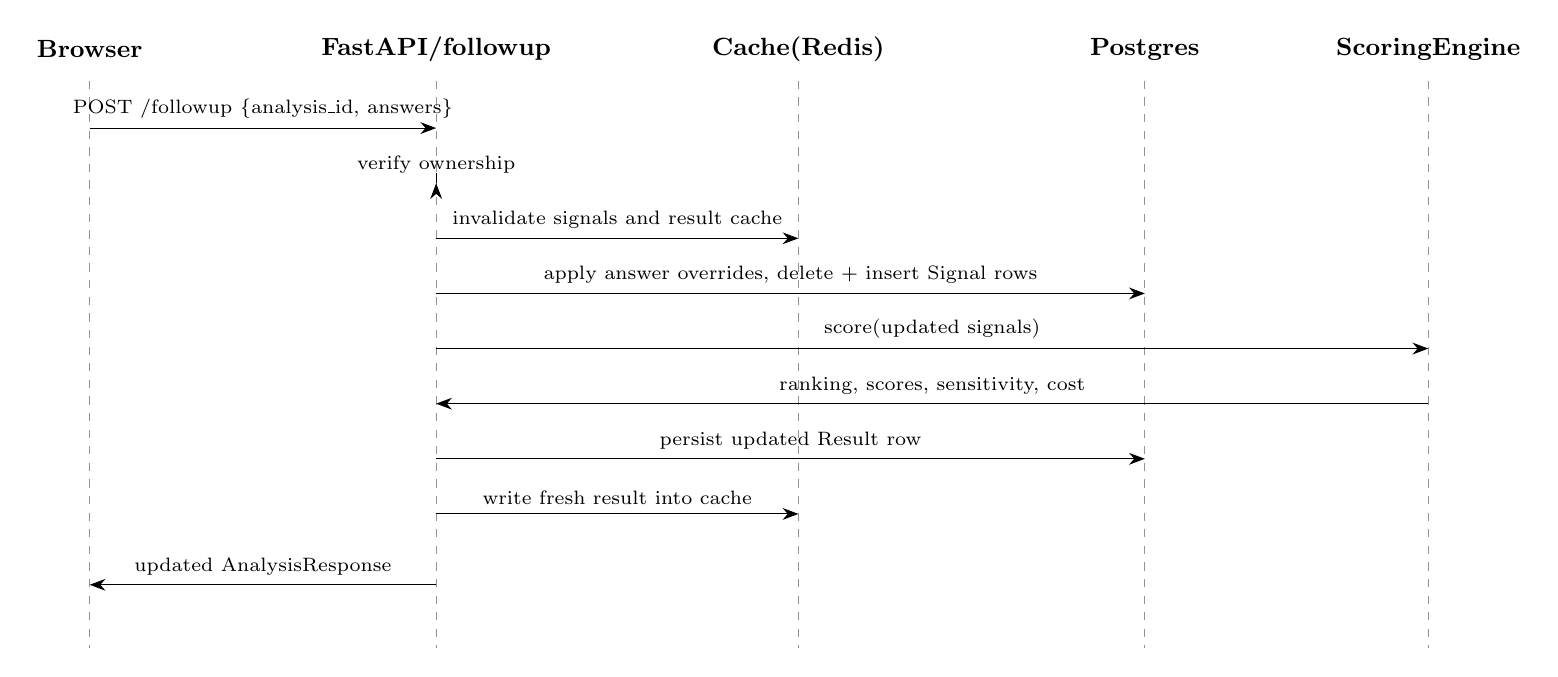
\begin{tikzpicture}[
  actor/.style={font=\small\bfseries},
  msg/.style={-{Stealth[length=2mm]}, font=\scriptsize},
  every node/.style={font=\scriptsize}
]
\node[actor] at (0,0) {Browser};
\node[actor] at (4.4,0) {FastAPI\\/followup};
\node[actor] at (9.0,0) {Cache\\(Redis)};
\node[actor] at (13.4,0) {Postgres};
\node[actor] at (17.0,0) {Scoring\\Engine};
\draw[dashed,darknavy!50] (0,-0.4) -- (0,-7.6);
\draw[dashed,darknavy!50] (4.4,-0.4) -- (4.4,-7.6);
\draw[dashed,darknavy!50] (9.0,-0.4) -- (9.0,-7.6);
\draw[dashed,darknavy!50] (13.4,-0.4) -- (13.4,-7.6);
\draw[dashed,darknavy!50] (17.0,-0.4) -- (17.0,-7.6);

\draw[msg] (0,-1.0) -- node[above]{POST /followup \{analysis\_id, answers\}} (4.4,-1.0);
\draw[msg] (4.4,-1.7) -- node[above]{verify ownership} (4.4,-1.7);
\draw[msg] (4.4,-2.4) -- node[above]{invalidate signals and result cache} (9.0,-2.4);
\draw[msg] (4.4,-3.1) -- node[above]{apply answer overrides, delete + insert Signal rows} (13.4,-3.1);
\draw[msg] (4.4,-3.8) -- node[above]{score(updated signals)} (17.0,-3.8);
\draw[msg] (17.0,-4.5) -- node[above]{ranking, scores, sensitivity, cost} (4.4,-4.5);
\draw[msg] (4.4,-5.2) -- node[above]{persist updated Result row} (13.4,-5.2);
\draw[msg] (4.4,-5.9) -- node[above]{write fresh result into cache} (9.0,-5.9);
\draw[msg] (4.4,-6.8) -- node[above]{updated AnalysisResponse} (0,-6.8);
\end{tikzpicture}
\end{center}

\textbf{Why cache invalidation happens before the database write, not after:} if a concurrent request for the same analysis arrived between the database write and the cache invalidation, it could read the old (now stale) cached value, persist it back into the cache after the invalidation ran, and "resurrect" stale data. Invalidating first, writing the new value last, and ensuring the new value is the last thing written closes this race condition window. A candidate should be able to reason through this kind of cache-database consistency ordering explicitly, as it is a frequent systems design interview topic.

\section{Retry Mechanisms}

Two distinct retry strategies exist in the codebase, each appropriate to its context. The frontend's authentication sync (`auth-context.tsx`) retries up to three times with exponential backoff, appropriate for a one-time, idempotent operation (upserting a user profile) where a brief delay is imperceptible to the user. The results page polling loop also uses exponential backoff (1.5 seconds, doubling toward a 15 second ceiling, capped at forty attempts), but this is not a "retry on failure" mechanism, it is a "poll until ready" mechanism, and the choice of exponential rather than fixed interval polling is specifically to balance responsiveness (fast initial polls catch quick analyses promptly) against server load (slow analyses do not generate constant, wasted traffic).

\chapter{State Management Deep Dive}

\section{State Ownership Map}

\begin{longtable}{p{4.0cm}p{3.4cm}p{4.6cm}}
\toprule
\textbf{State} & \textbf{Owned by} & \textbf{Lifetime and rationale} \\
\midrule
\endhead
Authenticated user object & React Context (`auth-context.tsx`) & Lives for the browser session; needed by many distant components (navbar, modals, API calls), changes infrequently, a textbook case for Context. \\
Cached ID token & Module level cache (`auth-token.ts`) & Four minute TTL; intentionally outside React's render cycle since it is a cross-cutting infrastructural concern, not UI state, and storing it in Context would cause unnecessary re-renders across the tree every time it refreshed. \\
Project list and metadata & `localStorage` plus backend (`projects-store.ts`) & Persists across sessions and reloads; synchronized to the backend for authenticated users (durable, cross device) and kept purely local for guests (no account to attach it to). \\
Per-project analysis history & `localStorage`, capped at ten entries per project & A lightweight, client side convenience feature; bounding its size prevents unbounded `localStorage` growth, a real and easily overlooked browser storage concern. \\
In-progress questionnaire answers & `localStorage`, keyed per project & Allows a user to navigate away and resume; namespacing the key per project prevents a returning guest's answers from colliding with a different project's saved answers. \\
Polling and progress UI state & Local component state (`useState`/`useEffect`) in the results page & Entirely ephemeral and specific to one page's lifecycle; would be wasteful and architecturally inappropriate to lift any higher. \\
Form input and modal visibility & Local component state & Classic, appropriately scoped UI state; React's own reconciliation handles re-renders efficiently at this granularity. \\
\bottomrule
\end{longtable}

\section{Why No Global State Library Was Used}

A candidate should be able to defend this choice confidently rather than apologize for it. Redux, Zustand, and similar libraries solve the problem of sharing and synchronizing state across many, deeply nested, frequently-updating components, and they introduce real costs: boilerplate, an additional concept for every team member to learn, and a temptation to centralize state that would be better left local. ArchGuide's actual cross-cutting state (the authenticated user) changes rarely and is well served by Context; its durable state (projects, history) is naturally suited to persistent storage (`localStorage` plus the backend database) rather than an in-memory store that would be lost on reload anyway; and its remaining state is naturally local to the component that uses it. Reaching for a global state library here would have been over-engineering, adding a dependency and a learning curve to solve a problem the codebase does not actually have. This is exactly the kind of judgment call (choosing the simplest tool that correctly fits the actual shape of the problem) that senior engineers look for.

\section{Rebuild and Re-render Mechanisms}

React re-renders a component when its own state changes, when a parent re-renders (by default, propagating downward), or when a consumed Context's value changes. The codebase shows explicit awareness of the performance implications of this: `ResultsDashboard` is wrapped in `React.memo` specifically because the results page polls repeatedly and would otherwise re-render the (relatively expensive, chart heavy) dashboard on every poll tick, even when the underlying data is unchanged; `React.memo` performs a shallow comparison of props and skips the re-render entirely when they are referentially equal, which is the case here because the polling logic only updates state (and therefore triggers a child re-render with new props) when the fetched data has actually changed.

\section{Memory Considerations}

The most notable client side memory consideration is the explicit ten-entry cap on per-project analysis history stored in `localStorage`; without it, a long lived, heavily used project could accumulate an unbounded amount of historical data in browser storage, eventually hitting the browser's per-origin storage quota (typically five to ten megabytes) and causing write failures. On the backend, the most notable memory consideration is the bounded LRU caches (the in-process L1 extraction cache at one thousand entries, and the sensitivity analysis cache), both explicitly designed to provide the performance benefit of caching without the risk of unbounded memory growth that an unbounded cache (a plain dictionary that is never cleaned up) would eventually cause, an important and frequently tested systems concept.

\chapter{Design Patterns Used}

\begin{longtable}{p{2.6cm}p{2.6cm}p{6.8cm}}
\toprule
\textbf{Pattern} & \textbf{Where used} & \textbf{Why used, benefits, and drawbacks} \\
\midrule
\endhead
Adapter & `LLMClient` (normalizes OpenAI, Groq, and Ollama APIs behind one interface); `PortableJSON` (normalizes `JSONB` versus `JSON` column types between PostgreSQL and SQLite) & \textbf{Why:} lets the rest of the system depend on one stable interface instead of several incompatible ones. \textbf{Benefit:} swapping or adding a provider or database backend requires changes in one place only. \textbf{Drawback:} the adapter itself can become a complexity hot spot if it tries to expose every provider-specific feature through the unified interface; this codebase wisely keeps the unified interface minimal (generate, generate\_json, chat, stream). \\
Strategy & `SignalExtractor`'s LLM-based versus heuristic-based extraction; `ScoringEngine`'s rule table driven scoring (behavior selected by data, not by conditional code branches) & \textbf{Why:} lets interchangeable algorithms be selected or substituted, including automatically at runtime on failure (the heuristic fallback). \textbf{Benefit:} new rules or extraction approaches can be added without restructuring the surrounding orchestration code. \textbf{Drawback:} can obscure control flow if overused; here it is applied only where genuine interchangeability exists. \\
Facade & `LLMClient` (hides token counting, truncation, retries, connection pooling, and streaming behind simple method calls); `recommendation_service.score\_and\_persist` (hides the multi-step scoring, sensitivity, cost, persistence, and caching sequence behind one call) & \textbf{Why:} gives calling code (routers) a simple, high level interface and keeps complex orchestration logic out of the HTTP layer, where it would be harder to test and reuse. \textbf{Benefit:} routers stay thin, readable, and focused on HTTP concerns. \textbf{Drawback:} a facade can become a "god object" if it accumulates too many responsibilities; this codebase mitigates that by further delegating to focused sub-services. \\
Cache-Aside (Lazy Loading) & `cache\_service`, `extraction\_cache` (check cache, on miss compute and populate) & \textbf{Why:} the simplest, most broadly applicable caching pattern, and appropriate when reads vastly outnumber writes, exactly the case for analysis results. \textbf{Benefit:} cache and source of truth (the database) cannot silently diverge in the way a write-through cache bug could cause; a cache failure simply means falling through to the source of truth. \textbf{Drawback:} the first request for any given key always pays the full computation cost (a "cold" miss); this is acceptable here because that cost is unavoidable for a genuinely new analysis anyway. \\
Repository-like Data Access & SQLAlchemy ORM models plus the `get\_db` dependency injected session & \textbf{Why:} separates the "what data do I need" (expressed as Python objects and queries) from "how is it physically stored and retrieved" (SQL, connection pooling), and makes the persistence layer mockable for tests (the test suite swaps in an in-memory SQLite engine transparently). \textbf{Benefit:} testability and the ability to evolve the underlying database technology with contained impact. \textbf{Drawback:} ORMs can hide expensive queries (the N+1 query problem the codebase explicitly fixed with an index, "B-11," is a classic example of this exact risk surfacing in practice). \\
Dependency Injection & FastAPI's `Depends()` mechanism (`get\_db`, `verify\_firebase\_token`, the rate limiter) & \textbf{Why:} lets route handlers declare what they need (a database session, an authenticated user) without constructing those things themselves, which is both cleaner and dramatically easier to test (dependencies can be overridden in tests, exactly as the test suite's `conftest.py` does to substitute a test database and a mocked authentication check). \textbf{Benefit:} loose coupling, high testability. \textbf{Drawback:} can make the source of a value less immediately obvious to a reader unfamiliar with the framework's conventions; mitigated by FastAPI's explicit, type-annotated `Depends()` syntax. \\
Singleton (module level shared instances) & The shared `httpx.AsyncClient` in `LLMClient`; the shared `limiter` instance in `app/limiter.py` (specifically structured to avoid circular imports) & \textbf{Why:} certain resources (HTTP connection pools, rate limiter state) are expensive to create and must be shared to be effective; creating a new one per request would defeat their purpose entirely. \textbf{Benefit:} connection reuse (measurable latency improvement, "B-02") and consistent, shared rate limiting state. \textbf{Drawback:} singletons can complicate testing (shared mutable state between tests) and obscure dependencies; the codebase mitigates this by keeping the singletons narrowly scoped to genuinely cross-cutting infrastructural concerns rather than business logic. \\
Memoization with LRU Eviction & Sensitivity analysis cache; extraction cache L1 layer & \textbf{Why:} the underlying computations are expensive and frequently repeated with identical inputs (the same document, the same signal configuration); caching trades memory for time, the classic and correct tradeoff when the computation is pure and repeatable. \textbf{Benefit:} dramatic latency and cost reduction on repeat access. \textbf{Drawback:} requires careful invalidation when inputs can change underneath the cache (handled here via explicit invalidation on follow-up answer changes) and bounded sizing to avoid unbounded memory growth (handled via LRU eviction). \\
Guard Clause / Gate Chain & `validate\_document\_relevance` (a sequence of independent, early-exit checks); the upload pipeline's confidence gating and concentration warning checks & \textbf{Why:} cheap checks should run, and reject bad input, before expensive work is attempted. \textbf{Benefit:} clearer code (each check is independently readable and testable) and better resource economics (fail fast, fail cheap). \textbf{Drawback:} a long chain of gates can become hard to reason about holistically if not well documented; this codebase keeps each gate's purpose explicit through naming and comments. \\
Observer (lightweight, via DOM events) & The `projects-updated` custom event dispatched on `window` whenever the project store changes, observed by pages that display project lists & \textbf{Why:} a minimal way to keep multiple, independently rendered parts of the UI synchronized with a shared, externally-persisted data source (`localStorage` plus the backend) without introducing a formal pub/sub library or global store. \textbf{Benefit:} zero additional dependencies, easy to understand for anyone familiar with the DOM event model. \textbf{Drawback:} less type-safe and discoverable than a formal state management solution's subscription model; appropriate at this scale, would need to be reconsidered if the number of cross-cutting events grew significantly. \\
\bottomrule
\end{longtable}

\chapter{Algorithms and Data Structures}

\section{Pre-compiled Regular Expression Keyword Matching}

\textbf{Where:} `signal\_extractor.py`'s keyword scoring and heuristic fallback engine.
\textbf{Explanation:} rather than calling `re.search()` (which compiles the pattern internally on every call) for each of dozens of keywords against each page of text on every extraction, the patterns are compiled exactly once at module load time and reused.
\textbf{Complexity analysis:} naive repeated compilation, for $p$ pages, $w$ keywords, and pattern compilation cost $C$, costs roughly $O(p \cdot w \cdot (C + n/p))$; pre-compilation removes the $C$ term from the inner loop, reducing the dominant cost to $O(p \cdot w \cdot n/p) = O(w \cdot n)$, a meaningful constant factor improvement at the scale of dozens of keywords across potentially hundreds of pages (this was explicitly measured and tagged as optimization "B-08" in the codebase).
\textbf{Alternatives:} a single combined regular expression with named groups (more complex to construct and to attribute matches back to specific keywords, but potentially faster still); a trie-based or Aho-Corasick multi-pattern matcher (asymptotically optimal for matching many fixed strings simultaneously, $O(n + z)$ where $z$ is the number of matches, but considerable additional implementation complexity for a problem of this modest scale).

\section{Sliding Window Chunking with Overlap}

\textbf{Where:} `embeddings.py`'s `chunk\_text` (token based, with a default window of 1024 tokens and 50 token overlap) and `signal\_extractor.py`'s character based chunking for long documents (5000 character windows).
\textbf{Explanation:} long documents must be split into pieces small enough to fit a model's context window or to keep individual LLM calls fast and cheap; overlap between consecutive windows ensures that a piece of information spanning a chunk boundary is not lost entirely from both chunks' perspectives.
\textbf{Complexity analysis:} producing $\lceil (n - o) / (s - o) \rceil$ chunks from an input of length $n$, with chunk size $s$ and overlap $o$, in $O(n)$ total time and $O(n \cdot s/(s-o))$ total space across all chunks (the overlap means total chunked content is somewhat larger than the original, by a factor that increases as overlap approaches chunk size).
\textbf{Alternatives:} sentence or paragraph boundary aware chunking (better semantic coherence per chunk, more complex to implement correctly across document formats); fixed, non-overlapping chunks (simpler and smaller, but risks losing boundary spanning information entirely).

\section{Least Recently Used (LRU) Cache via OrderedDict}

\textbf{Where:} the sensitivity analysis cache in `scoring\_engine.py` and the L1 layer of `extraction\_cache.py`.
\textbf{Explanation:} a Python `OrderedDict` is used to implement a fixed-capacity cache where, on a cache hit, the accessed entry is moved to the end (marking it most recently used), and when the cache exceeds its capacity, the entry at the front (least recently used) is evicted with `popitem(last=False)`.
\textbf{Complexity analysis:} both lookup-and-reorder and insertion-with-eviction run in amortized $O(1)$ time, because `OrderedDict` is backed by a hash map combined with a doubly linked list that tracks insertion and access order; space is bounded at $O(C)$ where $C$ is the configured capacity (one thousand entries for the extraction cache L1 layer).
\textbf{Alternatives:} `functools.lru\_cache` (a built-in decorator providing the same semantics for pure functions with hashable arguments, simpler to apply but less flexible for cases needing custom key construction or manual invalidation, both of which this codebase needs); a simple dictionary with manual timestamp tracking and periodic sweeps (higher constant factors, more code, more opportunities for subtle bugs).

\section{Weighted Linear Scoring with Confidence-Adjusted Contributions}

\textbf{Where:} `scoring\_engine.py`'s core `score()` algorithm.
\textbf{Explanation:} described in detail in Volume 1; in data structure terms, this is a weighted sum reduction over a small, fixed-size table lookup structure (effectively a three-dimensional associative array, signal name to signal value to architecture, implemented as nested Python dictionaries).
\textbf{Complexity analysis:} $O(k)$ where $k$ is the number of signals (a constant, ten), making this effectively $O(1)$ in practice; the nested dictionary lookups are each $O(1)$ expected time (Python dictionaries are hash maps).
\textbf{Alternatives:} a sparse matrix representation (would offer no benefit at this scale and would add unnecessary complexity); a trained linear or logistic regression model with learned weights (would replace hand-authored, auditable weights with opaque, data-derived ones, directly undermining the explainability goal that is central to this product's value proposition, see the discussion of this exact tradeoff in Chapter 19).

\section{Exponential Backoff Polling}

\textbf{Where:} the results page's analysis status polling loop.
\textbf{Explanation:} the interval between successive polls starts small (1.5 seconds) and doubles after each attempt, up to a ceiling (15 seconds), and the total number of attempts is capped (forty).
\textbf{Complexity analysis:} the total elapsed time before reaching the ceiling is a geometric series; the number of polls in the "ramping" phase before hitting the cap is $O(\log(\text{ceiling}/\text{initial}))$, after which polling continues at the fixed ceiling interval until either a result arrives or the overall attempt cap is reached. This balances responsiveness for fast analyses (frequent early polls) against server load for slow ones (infrequent later polls), and the hard cap bounds worst-case resource consumption from a single client to a known, finite quantity.
\textbf{Alternatives:} fixed-interval polling (simpler, but either wastes resources on fast analyses with a long fixed interval, or floods the server on slow ones with a short fixed interval); WebSockets or server-sent events for push-based status updates (would eliminate polling entirely and reduce latency to near real time, at the cost of additional infrastructure complexity, connection management, and the need to handle reconnection; a legitimate improvement to propose when discussing how this system could evolve, see Chapter 23 of Volume 3).

\chapter{Performance Analysis}

\section{Backend Bottlenecks}

\begin{enumerate}[leftmargin=*]
  \item \textbf{LLM API latency:} by far the largest single contributor to end-to-end analysis time; a single signal extraction call can take several seconds, and a long document may require several such calls (mitigated by parallel, semaphore-bounded chunk processing and by caching).
  \item \textbf{Synchronous database driver under an asynchronous framework:} `psycopg2` blocks the calling thread; FastAPI offloads synchronous dependency calls to a thread pool, which avoids stalling the event loop directly but introduces thread pool contention as a secondary bottleneck under high concurrent load.
  \item \textbf{PDF generation:} a CPU-bound, synchronous operation (FPDF performs no I/O but does substantial in-process layout computation for a multi-section, multi-page document); run inside an async route handler, a sufficiently large report could measurably delay the event loop, a candidate should be able to identify this as a place where offloading to a background worker or a thread pool would be a sensible improvement at higher load.
  \item \textbf{Vector search round trips:} each retrieval-augmented extraction requires an embedding generation call followed by a Qdrant search call, two sequential network round trips on the critical path of every document analysis.
\end{enumerate}

\section{Frontend Bottlenecks}

\begin{enumerate}[leftmargin=*]
  \item \textbf{Chart re-rendering during polling:} addressed via `React.memo` on `ResultsDashboard`, but a candidate should be able to explain why this was necessary (Recharts components perform non-trivial SVG layout computation on every render) and what would happen without it (visible jank and wasted CPU on every poll tick, even when displaying unchanged data).
  \item \textbf{Animated background and scroll effects:} Vanta.js (WebGL-based 3D rendering) and Framer Motion scroll transforms both consume meaningful CPU and GPU resources; mitigated by lazy loading the background effect (so it never blocks initial render) and by skipping scroll animations on mobile devices (where battery life and lower-powered GPUs make the cost-to-benefit ratio worse).
  \item \textbf{Bundle size:} a large dependency set (Firebase, Framer Motion, Recharts, Vanta, Lenis) risks a slow initial page load; mitigated by lazy loading Firebase (deferred until authentication is actually needed) and by `next.config.ts`'s explicit import optimization for `lucide-react`, `framer-motion`, and `recharts` (which enables tree-shaking of unused exports from these libraries).
\end{enumerate}

\section{Optimization Opportunities Going Forward}

\begin{itemize}[leftmargin=*]
  \item Migrate the database access layer to an async driver (`asyncpg`) and SQLAlchemy's async engine, removing the thread pool indirection entirely.
  \item Move PDF generation to a background task queue (for example, using FastAPI's `BackgroundTasks` for simple cases, or a dedicated task queue such as Celery or `arq` for heavier load), returning a "your report is being generated" response immediately and notifying the client when it is ready.
  \item Replace polling with WebSockets or server-sent events for analysis status updates, eliminating both the latency of the polling interval and the wasted requests during the "still processing" period.
  \item Pre-warm or pool embedding model connections similarly to how the Ollama HTTP client is already pooled, reducing the latency of the first vector operation in each analysis.
\end{itemize}

\begin{qabox}[Likely Interview Questions]
\textbf{Q: If a single document analysis is taking ninety seconds, how would you find out which stage is slow?} \\
A: The `decision\_trace` mechanism already timestamps every stage of the pipeline (parsing, validation, indexing, extraction, scoring) and is persisted with the result; this is effectively built-in, per-request distributed tracing at the application level. I would start by examining the trace for several slow analyses to see which stage's timestamps show the largest gaps, then drill into that stage specifically, for example, if extraction is slow, checking whether it is the LLM call itself (network and inference latency, visible in provider-side metrics or added instrumentation) or the chunking and merging logic around it (visible through application level profiling). This systematic, evidence-first approach, rather than guessing, is exactly what the existing decision trace was built to support.
\end{qabox}

\chapter{Scalability Analysis}

This chapter walks through what would happen, and what would need to change, as the user base grows by roughly one order of magnitude at each stage. The framing assumes the current architecture (a modular monolith on managed infrastructure) as the starting point.

\section{From 100 to 1,000 Users}

\textbf{What likely still works fine:} the current architecture, essentially unchanged. At this scale, request volume is low enough that a single backend instance, the existing rate limits, and the managed database, cache, and vector store free or low tiers comfortably absorb the load.

\textbf{What to watch:} LLM API costs become the first real budget line item worth monitoring closely, since they scale roughly linearly with the number of analyses performed; the caching layers (extraction cache, result cache) are precisely what keep this cost sub-linear in practice by avoiding redundant calls for repeated or reloaded analyses.

\section{From 1,000 to 10,000 Users}

\textbf{What starts to strain:}
\begin{itemize}[leftmargin=*]
  \item \textbf{Rate limiting state:} SlowAPI's default in-memory storage does not share state across multiple backend worker processes or instances; running more than one instance (which would likely become necessary around this scale to handle concurrent load) would mean each instance enforces its limits independently, effectively multiplying the real, system-wide limit by the instance count, an inconsistency that could allow abuse to slip through.
  \item \textbf{Database connection pool sizing:} the configured pool (ten persistent connections, twenty overflow) could become a contention point under sustained concurrent load from multiple backend instances all competing for the managed database's total connection limit.
  \item \textbf{Synchronous PDF generation inside async handlers} becomes more noticeable as concurrent export requests increase.
\end{itemize}

\textbf{What to change:} move rate limiting state to Redis (SlowAPI supports this via a Redis storage backend), so that all instances enforce a consistent, shared limit; consider a connection pooler such as PgBouncer in front of PostgreSQL to manage connections more efficiently across multiple backend instances; move PDF generation to a background task queue.

\section{From 10,000 to 100,000 Users}

\textbf{What breaks first and why:}
\begin{itemize}[leftmargin=*]
  \item \textbf{The synchronous database driver becomes a hard bottleneck:} at this scale, the thread pool that FastAPI uses to run synchronous dependencies becomes saturated under sustained load, and requests begin to queue waiting for a thread, directly increasing tail latency.
  \item \textbf{A single Redis instance's throughput} may become a contention point if it is serving as the backing store for caching, rate limiting, and (in a redesigned system) session or queue state simultaneously.
  \item \textbf{LLM provider rate limits} (imposed by OpenAI, Groq, and similar providers, independent of anything ArchGuide controls) become a real architectural constraint; the system would need request queuing, provider load balancing, and possibly negotiated higher-tier API agreements.
\end{itemize}

\textbf{What to change:} migrate to an async database driver and engine; horizontally scale backend instances behind a load balancer (made possible by the system's already-stateless authentication design, a significant existing strength); introduce a message queue (for example, RabbitMQ, AWS SQS, or Redis Streams) to decouple the expensive analysis pipeline from the request-response cycle entirely, an uploaded document would be queued, processed by a pool of worker processes, and the result delivered via push notification or polling against a lightweight status endpoint; this also naturally smooths out bursty load.

\section{From 100,000 to 1,000,000 Users}

\textbf{What breaks first and why:} a single managed PostgreSQL instance, however well tuned, has a ceiling on write throughput and storage; at this scale, the `Signal` and `Result` tables (which grow with every analysis ever run, by every user) would become very large, and queries that scan or aggregate across them would slow down without careful partitioning and archival strategy. The vector store would similarly need to handle a much larger and more diverse set of indexed documents, with attention to per-tenant (per-session) isolation at scale.

\textbf{What to change:} introduce read replicas for the database (the vast majority of this application's queries are reads, fetching projects, sessions, signals, and results, making read replicas a natural and high-leverage fit); consider partitioning or archiving old `Session`, `Signal`, and `Result` data (for example, moving analyses older than a configurable retention period to cold storage); introduce a Content Delivery Network (CDN) for the frontend's static assets (Vercel provides this natively, but it is worth being able to name explicitly); introduce comprehensive application performance monitoring and distributed tracing (extending the existing `decision\_trace` concept into a full observability stack, for example using OpenTelemetry); and seriously evaluate whether specific high-load components (for example, the signal extraction pipeline) should be extracted into independently scalable services, the first genuine step toward a microservices style decomposition, undertaken only once the monolith's internal boundaries have proven themselves stable and well-defined through real production experience, exactly the sequencing that experienced engineering organizations follow and that naive "microservices from day one" approaches typically get backwards.

\begin{qabox}[Likely Interview Questions]
\textbf{Q: At what user count would you start seriously considering microservices, and why not sooner?} \\
A: Roughly in the hundred-thousand-user range, and only for components that have demonstrated, through real production data, both a distinct scaling profile from the rest of the system and stable, well-understood boundaries, the signal extraction pipeline is the clearest candidate, since it is CPU and I/O intensive in a different way than, for example, simple project CRUD operations. Splitting too early carries real costs: network latency between services, distributed transaction complexity, duplicated infrastructure, and a substantially higher operational burden, all paid before there is any actual load to justify them. The right sequence is to build a well-modularized monolith first (which this codebase substantially is, with clearly separated routers and services), let real usage reveal where the genuine scaling pressure points are, and then extract precisely those points, not speculative ones, into independently scalable services.
\end{qabox}

\chapter{Production Readiness}

\section{What Exists Today}

\begin{itemize}[leftmargin=*]
  \item \textbf{Structured logging:} the codebase replaced ad hoc `print()` statements with proper logging calls (fix "SEC-004"), and suppresses overly verbose SQLAlchemy logging in production.
  \item \textbf{Health checks:} a dedicated `/api/v1/health` endpoint, the standard mechanism deployment platforms use to determine whether an instance is ready to receive traffic or needs to be restarted.
  \item \textbf{Crash recovery:} the startup lifespan handler detects and cleans up sessions orphaned by a previous crash, a notably mature touch for a project at this stage.
  \item \textbf{Containerization:} a `Dockerfile` exists for the backend, enabling consistent deployment across environments.
  \item \textbf{Platform-specific deployment configuration:} `railway.toml` for the backend and `vercel.json` for the frontend.
  \item \textbf{Database migrations:} a full Alembic migration history, enabling repeatable, versioned schema evolution.
  \item \textbf{Automated testing:} a real test suite on both backend (pytest, covering API endpoints, database integrity, security, and document analysis regressions) and frontend (Vitest, covering components and library functions).
  \item \textbf{Rate limiting and security headers:} discussed at length in Chapter 10.
\end{itemize}

\section{What Is Missing or Underdeveloped}

\begin{itemize}[leftmargin=*]
  \item \textbf{Application performance monitoring and distributed tracing:} beyond the application-level `decision\_trace`, there is no evidence of integration with an observability platform (for example, Datadog, New Relic, Honeycomb, or an OpenTelemetry-based stack) that would allow an on-call engineer to see, across the whole system and in real time, where time and errors are concentrated.
  \item \textbf{Centralized log aggregation and alerting:} structured logs exist, but there is no visible configuration for shipping them to a central system or for alerting on error-rate anomalies.
  \item \textbf{Continuous Integration / Continuous Deployment (CI/CD) pipeline definitions:} no GitHub Actions workflows, or equivalent CI configuration files, are present in the repository; tests exist but there is no visible automation that runs them on every push or pull request and gates deployment on their passing.
  \item \textbf{Frontend crash reporting and analytics:} no integration with a crash reporting service (for example, Sentry) or a product analytics platform is evident; the only error visibility is the `error.tsx` boundary's `console.error` call, which is invisible once the page is closed.
  \item \textbf{Secrets management strategy beyond environment variables:} `.env.example` files document the expected configuration shape, but there is no visible use of a dedicated secrets manager (for example, AWS Secrets Manager, HashiCorp Vault, or the hosting platform's equivalent) for rotating or auditing access to sensitive credentials in production.
  \item \textbf{Load testing artifacts:} no evidence of load or stress testing scripts or results, which would be the natural way to validate the scalability assumptions discussed in Chapter 17 before they are tested by real, unplanned production load.
\end{itemize}

\section{How HPE Engineers Would Likely Improve It}

A senior team inheriting this codebase for productionization at enterprise scale would likely, in rough priority order: (1) stand up centralized logging, monitoring, and alerting, since you cannot safely operate, or even respond to incidents in, a system you cannot observe; (2) introduce a CI/CD pipeline that runs the existing (already reasonably comprehensive) test suite on every change and blocks merges or deployments on failures, converting "we have tests" into "our tests actually protect us"; (3) add crash reporting and product analytics on the frontend, to know about user-facing failures before users have to report them manually; (4) formalize secrets management and access auditing, particularly important given that the system handles API keys for multiple paid LLM providers; and (5) conduct load testing to validate (or correct) the scalability assumptions in Chapter 17 with real data rather than analysis alone, then prioritize the resulting findings over speculative optimization.

\begin{notebox}[A note on framing this honestly in an interview]
A candidate should not be defensive about these gaps. The strongest possible answer to "what's missing for production?" is a clear-eyed, prioritized list very much like the one above, demonstrating that you understand what production-readiness actually requires, even in the parts of the system you have not yet built. Pretending the system is "basically done" when it visibly is not will read as a lack of judgment; calmly explaining what is missing, why it matters, and in what order you would address it reads as exactly the kind of engineering maturity a Full-Time Offer interview is designed to find.
\end{notebox}

\chapter{Engineering Tradeoffs}

For each major design decision, this chapter states the decision, the realistic alternatives that were available, and the tradeoffs actually involved, the kind of reasoning a candidate must be able to produce fluently and convincingly under questioning.

\section{Deterministic Rule-Based Scoring versus a Trained Machine Learning Model}

\textbf{Decision:} hand-author a rule table mapping signal values to architecture score deltas, combined with fixed importance weights.
\textbf{Alternative:} train a classifier or regression model on a labeled dataset of "correct" architecture decisions.
\textbf{Tradeoff:} the rule-based approach sacrifices the theoretical ability to discover subtle, non-obvious patterns that a sufficiently large labeled dataset might reveal, and requires manual effort to tune as understanding of the domain evolves. In exchange, it gains complete explainability (every score traces to a named rule), complete reproducibility (the same input always produces the same output, with no model drift over time or between deployments), and total independence from the practically nonexistent labeled training data this domain would require. For a product whose entire purpose is to help a human justify a decision to other humans, explainability is not a nice-to-have, it is the core value proposition, making this one of the most clearly correct tradeoffs in the entire codebase.

\section{Modular Monolith versus Microservices}

\textbf{Decision:} build one deployable FastAPI application with internally separated routers and services.
\textbf{Alternative:} decompose into independently deployable services (for example, a document processing service, a scoring service, a chat service) from the start.
\textbf{Tradeoff:} microservices offer independent scaling, independent deployment, and fault isolation between components, at the cost of network latency between services, distributed transaction complexity, duplicated infrastructure (each service needs its own deployment pipeline, monitoring, and often its own data store), and a substantially higher operational burden. At this project's actual scale (a small team, a moderate and not-yet-fully-understood load profile), that operational burden would dwarf any benefit; the modular monolith captures most of microservices' organizational benefit (clear internal boundaries that make the code easy to navigate, reason about, and eventually extract from) without paying any of their distributed-systems costs upfront. This is widely recognized as the correct default sequencing in the industry, and a candidate who can articulate exactly why, rather than simply asserting "monoliths are simpler," will stand out.

\section{Hybrid LLM and Heuristic Extraction versus LLM-Only Extraction}

\textbf{Decision:} run an LLM-based extractor first, and fall back to a fully deterministic, regular-expression-based heuristic extractor if it returns nothing usable.
\textbf{Alternative:} rely solely on the LLM, perhaps with retries.
\textbf{Tradeoff:} an LLM-only approach is simpler to build and maintain (one code path, one set of prompts to tune) but introduces a hard dependency on an external service's availability, speed, and output quality, any of which can fail independently and entirely outside the application's control. The hybrid approach roughly doubles the extraction logic that must be written and tested, but converts "the analysis fails" into "the analysis proceeds with somewhat lower confidence," a dramatically better failure mode for any user-facing product, and one that reflects a mature, defense-in-depth way of thinking about dependencies on systems you do not control.

\section{Synchronous SQLAlchemy versus an Async Database Driver}

\textbf{Decision:} use `psycopg2` (synchronous) with SQLAlchemy's standard, synchronous engine, inside an otherwise asynchronous FastAPI application.
\textbf{Alternative:} use `asyncpg` with SQLAlchemy's async engine and async session dependencies throughout.
\textbf{Tradeoff:} the synchronous approach is considerably simpler to write, debug, and reason about (no need to remember `await` on every database call, simpler stack traces, a much larger body of existing documentation and Stack Overflow answers to draw on), and FastAPI's automatic thread-pool offloading of synchronous dependencies absorbs the cost at low to moderate scale. The async approach removes that thread-pool indirection entirely and would meaningfully improve throughput at high concurrency, at the cost of a more complex programming model that the whole team must consistently apply correctly (a single accidentally-synchronous call in an async context can silently reintroduce the exact problem being solved). This is a textbook "premature optimization versus appropriate simplicity for current scale" tradeoff, and the synchronous choice, while it will eventually need revisiting (as discussed in Chapter 17), is a defensible one for a project at this stage, not a mistake.

\section{Multiple LLM Providers versus a Single Provider}

\textbf{Decision:} support OpenAI, Groq, and Ollama behind a unified `LLMClient` interface, selectable per request.
\textbf{Alternative:} commit to a single provider.
\textbf{Tradeoff:} multi-provider support roughly doubles or triples the surface area that must be tested and maintained (different APIs, different error formats, different streaming protocols, different quality and latency characteristics to tune prompts against), but buys resilience against any single provider's outage or policy change, cost flexibility (free or near-free options for development and lower-stakes use, premium options for production-quality output), and the ability to let users make their own cost-versus-quality choice. For a project still establishing its product-market fit and operating under real budget constraints, this flexibility is valuable; a more mature, scaled product might eventually consolidate around whichever provider proves most cost-effective at its actual usage volume, trading flexibility for reduced maintenance burden, exactly the kind of "evolve the tradeoff as the context changes" thinking a senior engineer should be able to articulate.

\section{Vanta.js and Heavy Animation versus a Lean, Minimal Interface}

\textbf{Decision:} invest meaningfully in visual polish (3D animated backgrounds, scroll-driven animations, smooth scrolling, transition animations) on the marketing and dashboard surfaces.
\textbf{Alternative:} a deliberately minimal, fast-loading, low-animation interface (in the style of, for example, a developer tool or an internal enterprise dashboard).
\textbf{Tradeoff:} visual polish meaningfully increases bundle size, runtime resource consumption, and the surface area for performance regressions, and contributes nothing to the product's core analytical value. It does, however, materially affect a first-time visitor's perception of the product's quality and trustworthiness, "does this look like something built by people who care about details," which matters disproportionately for a product whose entire pitch is about making careful, well-reasoned, trustworthy decisions. The codebase shows clear awareness of this tension (lazy loading the background effect, skipping animations on mobile, optimizing imports), suggesting the polish was added thoughtfully rather than carelessly, a nuance worth pointing out if asked to critique this choice.

\end{document}
